\chapter{Soporte de Turtlebot 2 en ROS Foxy}
\label{cap:capitulo4}

% -- INTRODUCCION
% -----------------
En este capítulo se presenta el proceso de migración del robot Turtlebot2 de \textit{ROS Noetic} a \textit{ROS Foxy}. Se describirán todos los cambios relevantes realizados como puede ser la modificación de sus ficheros URDF/Xacro, su lanzamiento en Gazebo a través de los launchers de ROS2 o incluso su integración sobre una imagen Docker.\\

El soporte más estable del Turtlebot2 se encuentra en la rama de \textit{ROS Melodic} (tanto real como simulado) aunque también funciona en ROS Noetic \footnote{\textbf{Turtlebot 2 (Noetic)}: \url{https://bitbucket.org/theconstructcore/turtlebot/src/noetic/}}. Sin embargo, para ROS2 Foxy solamente hay un repositorio \footnote{\textbf{Base Kobuki (foxy)}: \url{https://github.com/kobuki-base/kobuki_ros}} con los drivers para mover la base kobuki [\ref{sec:kobuki_base}] real (sin  ficheros de lanzamiento para Gazebo).\\

De modo que el primer paso del proyecto fue dar soporte completo al Turtlebot2 en ROS Foxy para poder desarrollar los nuevos ejercicios de Robotics Academy. A continuación mostraré en orden los pasos realizados hasta su resultado final.\\


% -- SECCION KOBUKI BASE
% ------------------------
\section{Base Kobuki}
\label{sec:kobuki_base}

El respositorio oficial de kobuki base contiene los siguientes paquetes relevantes:

\begin{itemize}
	\item \textbf{kobuki\_description}: Es el paquete que contiene los ficheros de descripción xacro [\ref{subsec:xacro}] y URDF [\ref{subsec:urdf}] de la base. Con este directorio se describe el árbol de tranformadas que existen entre todos los \textit{links} del robot, y de esta manera poder conocer la localización de todos los frames. También se añaden \textit{plugins} para facilitar el control de movimiento del robot (controladores de velocidad, odometría ...).
	\item \textbf{kobuki node}: Es el paquete que contiene un fichero de configuración denominado \textit{kobuki\_node\_params.yaml} con el que podemos conectarnos al robot real usando el puerto /dev/ttyUSB0, así como la definición de algunos frames (base, odom). También contiene los ficheros de los nodos necesarios para controlar la base \textit{Kobuki} y su odometría. Oculta al programador la complejidad de comunicarnos directamente con el hardware (motores, leds...) del robot usando nodos ROS (usando publicadores y suscriptores). El nodo que lanza \textit{kobuki\_ros\_node} se suscribe al tópic /commands/velocity para recibir mensajes de tipo \textit{geometry\_msgs.msg.Twist} y poder mover mediante velocidad lineal y angular la base del robot. Este directorio no tiene relación con \textit{kobuki\_description}.
	\item \textbf{kobuki\_keyop}: Es un paquete que nos permite mover la base del robot con el teclado del ordenador. Se crea un nodo que publica por cada pulsación del teclado, un mensaje geometry\_msgs.msg.Tiwst en el topic /cmd\_vel (tendremos que cambiar a /commands/velocity si queremos controlar el robot real. Este paquete nos puede ayudar en un principio a comprobar que tenemos conexión con el hardware real.
\end{itemize}

Con estos 3 paquetes tenemos lo necesario para controlar la base del robot. Sin embargo, solo nos sirve para el robot real, y no en simulado. Como se ha mencionado antes, el paquete \textit{kobuki\_description} no tiene relación con kobuki\_node, solo nos permite visualizar un árbol de transformadas con el visualizador \textit{RVIZ 2} de modo que el siguiente paso fue representar la base Kobuki, mediante los ficheros de descripción, en un escenario de Gazebo.\\




% -- SECCION LANZAMIENTO EN GAZEBO
% ----------------------------------
\subsection{Lanzamiento en Gazebo}
\label{subsec:kobuki_gazebo}

Para conseguir la representación de la base kobuki en Gazebo hicimos un \textit{fork}\footnote{\textbf{Kobuki ROS (fork)}: \url{https://github.com/Carlosalpha1/kobuki_ros}} del repositorio oficial e implementamos un nuevo paquete llamado \textit{kobuki\_gazebo}. Dentro se incluyeron ficheros \textit{launch.py} para lanzar tanto el simulador como la base kobuki simulada. A continuación describiremos los ficheros más importantes del nuevo paqueté implementado:

\begin{itemize}
	\item \textbf{empty\_world.launch.py}: Un punto de partida en muchas ocasiones cuando creamos un robot simulado es diseñar un fichero de lanzamiento que únicamente lance un mundo vacío en Gazebo. De esta manera, puedes incluir ese fichero en otros ficheros de lanzamiento y dividimos un problema complejo en varios subproblemas. Para lanzar \textit{Gazebo} en ROS2 ejecutamos dos ficheros de lanzamientos en este orden:
	\begin{enumerate}
		\item gazebo\_ros - gzserver.launch.py: Lanza un servidor de Gazebo sin ventana, permitiendo ejecutar programas sin necesidad de visualizar el resultado en el simulador.
		\item gazebo\_ros - gzclient.launch.py: Lanza un cliente gazebo que activa una ventana donde podemos ver el mundo solicitado.
	\end{enumerate}
	
	\cleardoublepage
\begin{code}[H]
\begin{lstlisting}[frame=single]
def generate_launch_description():

	ld = LaunchDescription()

	pkg_gazebo_ros = get_package_share_directory('gazebo_ros')
		
	gazebo_server = IncludeLaunchDescription(
		PythonLaunchDescriptionSource(os.path.join(pkg_gazebo_ros, 'launch', 'gzserver.launch.py'))
	)
		
	gazebo_client = IncludeLaunchDescription(
		PythonLaunchDescriptionSource(os.path.join(pkg_gazebo_ros, 'launch', 'gzclient.launch.py'))
	)
	
	ld.add_action(gazebo_server)
	ld.add_action(gazebo_client)
	
	return ld
\end{lstlisting}
\caption[kobuki\_gazebo: empty\_world.launch.py]{kobuki\_gazebo: empty\_world.launch.py}
\label{cod:kobuki_gazebo_empty_world}
\end{code}

	\item \textbf{spawn\_model.launch.py}: Este fichero pasa los datos de descripción \textit{urdf} de la base \textit{Kobuki} a un parámetro denominado \textit{/robot\_description}, publica el estado del robot, sus transformadas y ejecuta el fichero de gazebo\_ros spawn\_entity.py para visualizar el modelo en el simulador:
	
\begin{code}[H]
\begin{lstlisting}[frame=single]
kobuki_model = Node(
	package='robot_state_publisher',
	executable='robot_state_publisher',
	parameters=[{'robot_description': robot_desc}],
	arguments=[urdf_file]
)

joint_state_publisher_node = Node(
	package='joint_state_publisher',
	executable='joint_state_publisher',
	name='joint_state_publisher'
)

spawn_entity = ExecuteProcess(
	cmd=['ros2', 'run', 'gazebo_ros', 'spawn_entity.py', '-topic', '/robot_description', '-entity', 'kobuki'], output='screen')
\end{lstlisting}
\caption[kobuki\_gazebo: spawn\_model.launch.py]{kobuki\_gazebo: spawn\_model.launch.py}
\label{cod:kobuki_gazebo_spawn_model}
\end{code}
\end{itemize}

Podemos visualizar la base \textit{Kobuki} en el simulador ejecutando los siguientes comandos:\\

\begin{code}[H]
\begin{lstlisting}
ros2 launch kobuki_gazebo empty_world.launch.py &
ros2 launch kobuki_gazebo spawn_model.launch.py
\end{lstlisting}
\caption{Comandos para lanzar la base Kobuki en Gazebo}
\label{cod:comandos_kobuki_launch}
\end{code}\

En la figura \ref{fig:sim_kobuki_base} podréis ver el resultado de la base \textit{Kobuki} en Gazebo
\begin{figure} [H]
  \begin{center}
    \includegraphics[width=10cm]{imagenes/sim_kobuki_base.png}
  \end{center}
  \caption[Modelo simulado Kobuki (ROS2)]{Modelo simulado Kobuki (ROS2)}
  \label{fig:sim_kobuki_base}
\end{figure}\




% -- SECCION IMAGEN DOCKER
% --------------------------
\subsection{Imagen Docker}
\label{subsec:kobuki_base_docker}

Para empezar a controlar la base Kobuki con un contenedor \textit{docker}, definimos un fichero Dockerfile con todas las dependencias necesarias junto con los comandos necesarios para lanzar los nodos.\\

En esta dirección, podréis descargar una versión de prueba que desarrollamos para mover un robot real Turtlebot2 en ROS Foxy con el paquete \textit{kobuki\_keyop} sin necesidad de instalar ROS2 ni ninguna otra dependencia: \url{https://hub.docker.com/r/carlosalpha1/kobuki_keyop}. Al lanzar el contenedor se muestra una ventana emergente del terminal \textit{xterm} para pulsar las teclas correspondientes que moverán la base del robot.\\

\textbf{Comandos para lanzar el contenedor kobuki\_base}:\\
\begin{code}[H]
\begin{lstlisting}
xhost +
docker run -it --rm --device /dev/ttyUSB0 -e DISPLAY=$DISPLAY -v /tmp/.X11-unix:/tmp/.X11-unix carlosalpha1/kobuki_keyop:ros-foxy
xhost -
\end{lstlisting}
\caption{Comando de lanzamiento del contenedor de prueba \textit{Kobuki\_Keyop} (ROS2)}
\label{cod:comando_kobuki_keyop_docker}
\end{code}\

Controlar la base kobuki supone un avance muy significativo para poder usar el robot Turtlebot2. Solamente haría falta usar paquetes de ROS para el láser y la cámara (tal y como veremos en el capítulo [\ref{cap:capitulo6}]). Sin embargo, aún no tenemos disponible la simulación completa del robot Turtlebot2, por lo que en los siguientes apartados integraremos la estructura que soporta la base.\\




% -- SOPORTE TURTLEBOT 2
% ------------------------
\section{Soporte Turtlebot 2}
\label{sec:soporte_turtlebot2}

A parte de la base Kobuki, la otra mitad que caracteriza al Turtlebot2 es la \textbf{base superior} que permite colocar portátiles, sensores o actuadores. En esta sección abordaremos su modelado y simulación con URDF y Xacro para ROS Foxy.

La pregunta es ¿por qué no usamos ficheros turtlebot\_description de la rama Noetic o Melodic si el lenguaje URDF es el mismo? En realidad, el paso de ROS a ROS2 conlleva cambios tanto en la manera de crear nodos, ficheros de lanzamiento y su funcionamiento interno como en el uso de URDF. El modelo Turtlebot2, al tener una gran cantidad de ficheros URDF que dependían unos de otros, y estos a su vez de otros paquetes con dependencias en ROS, no facilitaba la tarea de obtener un modelo creando únicamente ficheros de lanzamiento launch.py como hicimos con la base Kobuki.\\

Entonces, la \textit{solución} fue crear la estructura restante del robot a mano, usando la sintáxis URDF y Xacro, diseñando un modelo lo más semejante posible al real. A continuación mostraremos las fases de desarrollo. Una vez terminado el modelo del Turtlebot2, tendremos por un lado un directorio con todos los paquetes de kobuki\_base y otro directorio con la definición del nuevo soporte creado.\\



% -- FICHEROS DE CONFIGURACION XACRO
% ------------------------------------
\subsection{Ficheros de Configuración XACRO}
\label{subsec:turtlebot2_xacro}

El primer paso de esta segunda parte fue crear el modelo URDF. Usando Xacro nos permitió diseñar \textit{macros} que facilitara la estructura y la legibilidad del modelo. Con Xacro ha resultado sencillo incluir nuevos elementos en el modelo y establecer la jerarquía de transformadas entre \textit{links} de padres a hijos (siempre es importante indicar las relaciones jerárquicas para poder realizar futuras operaciones basadas en frames).\\

La estructura del nuevo directorio es la siguiente:
\begin{figure}[H]
	\begin{center}
	    \setlength{\fboxsep}{0.5cm}
	    \fbox{
        \begin{minipage}{10cm}
          \dirtree{%
          .1 turtlebot2.
          .2 kobuki\_base.
          .3 kobuki\_ros\_interfaces.
          .3 kobuki\_ros.
          .4 Ficheros de kobuki\_gazebo \ref{subsec:kobuki_gazebo}.
          .4 \vdots.
          .2 turtlebot2.
          .3 launch.
          .4 empty\_world.launch.py.
          .4 spawn\_model.launch.py.
          .3 rviz.
          .3 urdf.
          .4 structures.urdf.xacro.
          .4 colors.urdf.xacro.
          .4 turtlebot2.urdf.xacro.
          .4 sensors.
          .5 camera.urdf.xacro.
          .5 lidar.urdf.xacro.
          .3 spawn.sh.
          .3 CMakeLists.txt.
          .3 package.xml.
          }
        \end{minipage}
        }
	    \caption{Estructura de directorios completa del Turtlebot2 (ROS2 Foxy)}
	    \label{fig:directorios_turtlebot2}
	\end{center}
\end{figure}

En el fichero \textit{colors.urdf.xacro} definimos algunas macros para incluir colores en los \textit{links} del modelo de Gazebo:\\
\begin{code}[H]
\begin{lstlisting}
<xacro:macro name="create_color" params="name value">
	<material name="${name}">
		<color rgba="${value}"/>
	</material>
</xacro:macro>

<xacro:macro name="gazebo_color" params="link color">
	<gazebo reference="${link}">
		<material>Gazebo/${color}</material>
	</gazebo>
</xacro:macro>

<xacro:create_color name="Gray" value="0.5 0.5 0.5 1"/>
<xacro:gazebo_color link="base_tick1_link" color="Gray"/>
\end{lstlisting}
\caption{Creación y establecimiento de un color a un \textbf{link}}
\label{fig:creacion_color_link}
\end{code}\

En el fichero \textit{structures.urdf.xacro} definimos dos macros para crear los \textit{links} que necesitamos y definimos las relaciones jerárquicas de padres a hijos. Las nuevas macros son \textit{cylinder\_structure} y \textit{cube\_structure}, para crear en el fichero turtlebot2.urdf.xacro elementos como los siguientes:
\begin{code}[H]
\begin{lstlisting}
<xacro:cylinder_structure name="base_tick5" x="0.15" y="0.0" z="0.14" length="0.15" radius="0.005" parent="base_link"/>
<xacro:cube_structure name="camera_support_base" x="0.13" y="0" z="0.0975" x_size="0.0175" y_size="0.15" z_size="0.005" parent="middle_base_link"/>
\end{lstlisting}
\caption{Creación de dos links usando dos nuevas macros definidas (Turtlebot2 ROS Foxy)}
\label{fig:creacion_link_macro}
\end{code}

En el fichero \textit{turtlebot2.urdf.xacro} incluimos con la macro ``xacro:include" las definiciones URDF de los ficheros del paquete kobuki\_description. Por último, creamos dos ficheros XACRO para colocar una cámara RGBD y un láser 360 grados. Los ficheros de los sensores los podéis ver en este \textit{enlace}. \footnote{\textbf{Sensores Turtlebot2}: \url{https://github.com/RoboticsLabURJC/2021-tfg-carlos-caminero/tree/main/turtlebot2/turtlebot2/urdf/sensors/}}\\

Mediante este comando podemos generar un fichero urdf con toda la descripción del modelo a partir de turtlebot2.urdf.xacro:\\
\begin{code}[H]
\begin{lstlisting}
ros2 run xacro xacro urdf/turtlebot2.urdf.xacro > urdf/turtlebot2.urdf
\end{lstlisting}
\caption{Comando para convertir Xacro a URDF}
\label{fig:comando_xacro_2_urdf}
\end{code}




% -- TURTLEBOT 2: LANZAMIENTO EN GAZEBO
% ---------------------------------------
\subsection{Lanzamiento en Gazebo}
\label{subsec:turtlebot2_gazebo}

Para la visualización del modelo URDF completo en Gazebo me basé en los mismos ficheros que hice con la base Kobuki: empty\_world.launch.py y spawn\_model.launch.py [\ref{subsec:kobuki_gazebo}]\\

La única diferencia fue definir 3 argumentos por defecto para establecer la posición inicial del robot, y poder especificar el punto de partida cuando se quiera importar el modelo en cualquier otro mundo de Gazebo. Estos 3 argumentos se pasan al nodo spawn\_entity. A continuación podemos ver la sección referente a la posición inicial del fichero \textit{spawn\_model.launch.py}:\\

\begin{code}[H]
\begin{lstlisting}
	# Set (x, y, z) default position of turtlebot2
	x_pos = LaunchConfiguration('-x', default='0')
	y_pos = LaunchConfiguration('-y', default='0')
	z_pos = LaunchConfiguration('-z', default='0')
	
	spawn_entity_node = Node(
		package='gazebo_ros',
		executable='spawn_entity.py',
		name='entity_spawner',
		output='screen',
		arguments=["-topic", "/robot_description", "-entity", "turtlebot2", "-x", x_pos, "-y", y_pos, "-z", z_pos]
	)
\end{lstlisting}
\caption{Establecimiento de la posición por defecto del Turtlebot2 en el simulador}
\label{cod:posicion_defecto_turtlebot2_simulador}
\end{code}\

Para lanzar el modelo en el simulador ejecutamos los siguientes comandos:\\
\begin{code}[H]
\begin{lstlisting}
ros2 launch turtlebot2 empty_world.launch.py &
ros2 launch turtlebot2 spawn_model.launch.py
\end{lstlisting}
\caption{Comandos para lanzar el robot Turtlebot2 en el simulador (ROS2 Foxy)}
\label{codd:comandos_turtlebot2_simulador}
\end{code}

En la figura \ref{fig:evolucion_turtlebot2_sim} podemos ver la evolución del proceso creativo del Turtlebot 2 simulado:
\begin{figure} [H]
  \begin{center}
    \includegraphics[width=10cm]{imagenes/creacion-turtlebot2-sim.png}
  \end{center}
  \caption[Evolución Turtlebot 2 simulado]{Evolución Turtlebot 2 simulado}
  \label{fig:evolucion_turtlebot2_sim}
\end{figure}\


\textbf{Consideraciones a tener en cuenta}: Tanto el modelo Kobuki como el Turtlebot 2 simulado usan un plugin para controlar los motores denominado \textit{differential\_drive\_controller.so}. Este plugin se suscribe a un topic para controlar la velocidad de las ruedas del robot llamado /cmd\_vel (estándar en ROS), por lo que no coincide con el topic del robot real /commands/velocity.


